\RequirePackage{luatex85}
\documentclass{standalone}
\usepackage{tikz}

% Color Definitions
\definecolor{SourceColor}{RGB}{85,168,104}
\definecolor{TargetColor}{RGB}{221,132,82}
\definecolor{TargetChangerColor}{RGB}{255,153,0}
\definecolor{AbsorbingAreaColor}{RGB}{196,78,82}
\definecolor{ObstacleColor}{RGB}{179,179,179}
\definecolor{StairColor}{RGB}{129,114,178}
\definecolor{MeasurementAreaColor}{RGB}{255,0,0}
\definecolor{InformationAreaColor}{RGB}{0,100,20}
\definecolor{AerosolCloudColor}{RGB}{202,156,76}
\definecolor{AgentColor}{RGB}{76,114,202}
\definecolor{AgentIdColor}{RGB}{255,127,0}

\newcommand{\MeasurementAreaOpacity}{0.549020}
\newcommand{\AerosolCloudOpacity}{0.039216}

\begin{document}
\begin{tikzpicture}
\node[inner sep=0pt] (russell) at (0,0)
% Answer: [trim={left bottom right top},clip]
    {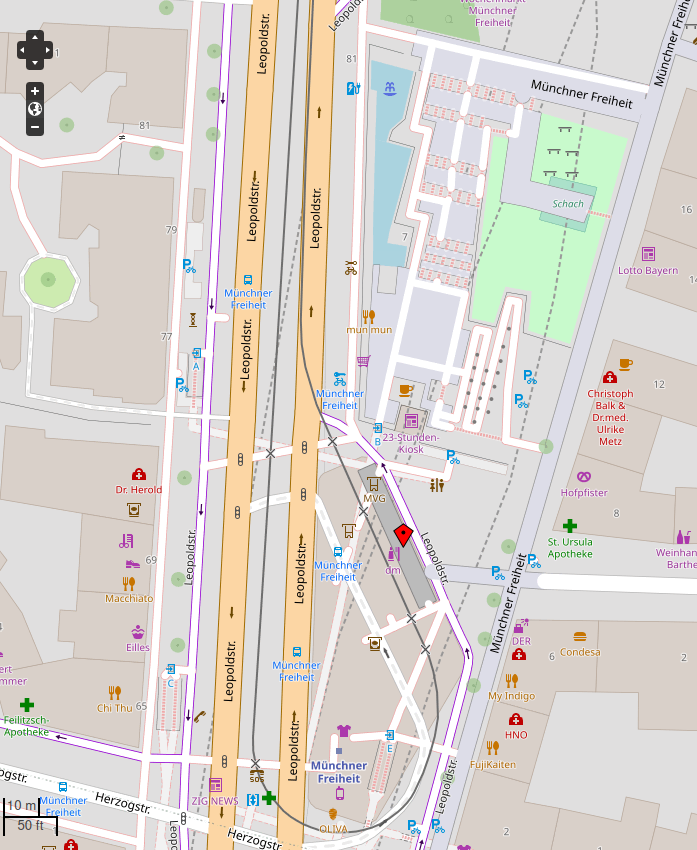
\includegraphics[width=7cm, trim={10.5cm 6cm 1cm 1cm},clip]{./openstreetmap.png} };
\node[inner sep=0pt] (whitehead) at (7.6,0)
    {\includegraphics[width=7cm, trim={51cm 5cm 30cm 0},clip]{./tikz/realistic_route_choice.pdf}};
\draw[->] (5.5,-2.8) -- (4.6,-1) -- (4.6,5.7) -- (6,5.3) -- (5.2,-0.7);
\draw[->] (5.5,-2.8) -- (5.7,-3.6) -- (5.7,-5.8);
\draw[->] (5.5,-2.8) -- (7.4,-1.6) -- (7.4,-1) --  (6.2,-1) -- (6.1,0.0) -- (5.3,0.0) -- (5.2,-0.7);
\node[] at (8.7,-1.2) {Medium route};
\node[text width=3cm] at (7.6,4.7) {Long route  (to \\ be recommended)};
\node[text width=2cm] at (7.2,-4.8) {Short route \\ (congested)};
\node[text width=1.8cm] at (5.8,-2.5) [fill=olive] {Arrivals \\ (bus/tram)};
\node at (6.2,-5.8) [fill=blue] {U};
\node at (5.7,-0.8) [fill=blue] {U};
\draw[->, red] (5.65,-5.4) -- (5.65,-4);
\node[red] at (4.4,-4.8) {Counterflow};
\end{tikzpicture}
\end{document}
